\documentclass[14pt]{extbook}
\usepackage{multicol, enumerate, enumitem, hyperref, color, soul, setspace, parskip, fancyhdr} %General Packages
\usepackage{amssymb, amsthm, amsmath, bbm, latexsym, units, mathtools} %Math Packages
\everymath{\displaystyle} %All math in Display Style
% Packages with additional options
\usepackage[headsep=0.5cm,headheight=12pt, left=1 in,right= 1 in,top= 1 in,bottom= 1 in]{geometry}
\usepackage[usenames,dvipsnames]{xcolor}
\usepackage{dashrule}  % Package to use the command below to create lines between items
\newcommand{\litem}[1]{\item#1\hspace*{-1cm}\rule{\textwidth}{0.4pt}}
\pagestyle{fancy}
\lhead{Progress Quiz 4}
\chead{}
\rhead{Version A}
\lfoot{4378-7085}
\cfoot{}
\rfoot{Fall 2020}
\begin{document}

\begin{enumerate}
\litem{
Describe the end behavior of the polynomial below.\[ f(x) = 9(x - 2)^{2}(x + 2)^{7}(x + 3)^{4}(x - 3)^{5} \]\begin{enumerate}[label=\Alph*.]
\begin{multicols}{2}\item 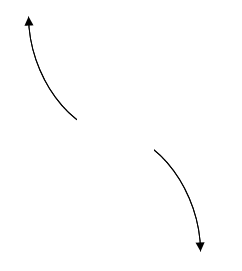
\includegraphics[width = 0.3\textwidth]{../Figures/polyEndBehaviorAA.png}\item 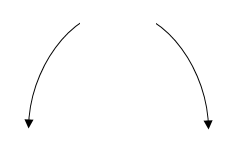
\includegraphics[width = 0.3\textwidth]{../Figures/polyEndBehaviorBA.png}\item 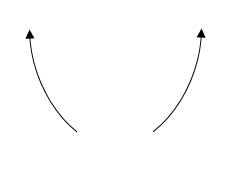
\includegraphics[width = 0.3\textwidth]{../Figures/polyEndBehaviorCA.png}\item 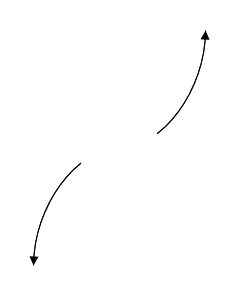
\includegraphics[width = 0.3\textwidth]{../Figures/polyEndBehaviorDA.png}\end{multicols}\item None of the above.
\end{enumerate} }
\litem{
Describe the zero behavior of the zero $x = 3$ of the polynomial below.\[ f(x) = -4(x - 8)^{5}(x + 8)^{4}(x - 3)^{8}(x + 3)^{5} \]\begin{enumerate}[label=\Alph*.]
\begin{multicols}{2}\item 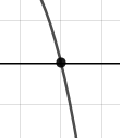
\includegraphics[width = 0.3\textwidth]{../Figures/polyZeroBehaviorCopyAA.png}\item 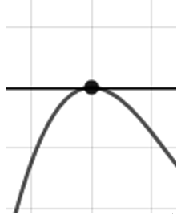
\includegraphics[width = 0.3\textwidth]{../Figures/polyZeroBehaviorCopyBA.png}\item 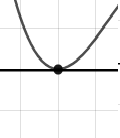
\includegraphics[width = 0.3\textwidth]{../Figures/polyZeroBehaviorCopyCA.png}\item 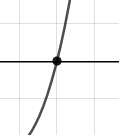
\includegraphics[width = 0.3\textwidth]{../Figures/polyZeroBehaviorCopyDA.png}\end{multicols}\item None of the above.
\end{enumerate} }
\litem{
Describe the zero behavior of the zero $x = -3$ of the polynomial below.\[ f(x) = 9(x + 3)^{5}(x - 3)^{10}(x - 6)^{8}(x + 6)^{11} \]\begin{enumerate}[label=\Alph*.]
\begin{multicols}{2}\item 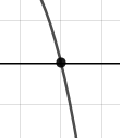
\includegraphics[width = 0.3\textwidth]{../Figures/polyZeroBehaviorAA.png}\item 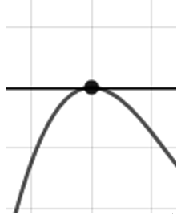
\includegraphics[width = 0.3\textwidth]{../Figures/polyZeroBehaviorBA.png}\item 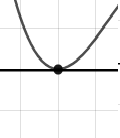
\includegraphics[width = 0.3\textwidth]{../Figures/polyZeroBehaviorCA.png}\item 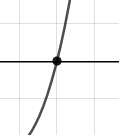
\includegraphics[width = 0.3\textwidth]{../Figures/polyZeroBehaviorDA.png}\end{multicols}\item None of the above.
\end{enumerate} }
\litem{
Construct the lowest-degree polynomial given the zeros below. Then, choose the intervals that contain the coefficients of the polynomial in the form $x^3+bx^2+cx+d$.\[ 5 - 2 i \text{ and } -1 \]\begin{enumerate}[label=\Alph*.]
\item \( b \in [-1, 7], c \in [0, 8], \text{ and } d \in [2, 6] \)
\item \( b \in [-1, 7], c \in [-9, -3], \text{ and } d \in [-5, -2] \)
\item \( b \in [-9, -6], c \in [15, 20], \text{ and } d \in [25, 36] \)
\item \( b \in [6, 16], c \in [15, 20], \text{ and } d \in [-30, -27] \)
\item \( \text{None of the above.} \)

\end{enumerate} }
\litem{
Which of the following equations \textit{could} be of the graph presented below?
\begin{center}
    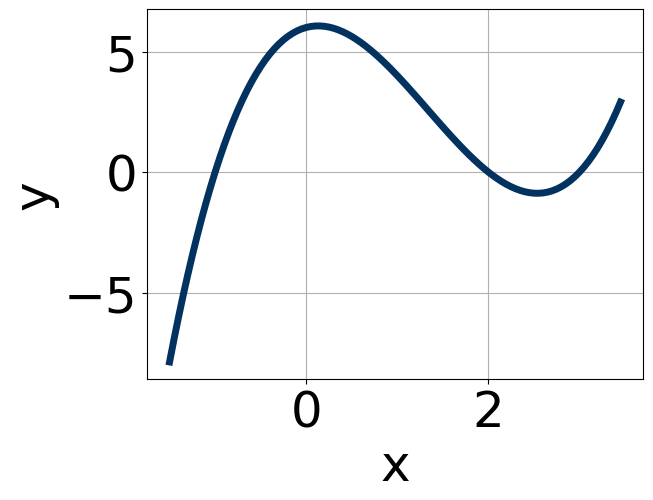
\includegraphics[width=0.5\textwidth]{../Figures/polyGraphToFunctionCopyA.png}
\end{center}
\begin{enumerate}[label=\Alph*.]
\item \( -14(x - 3)^{8} (x - 2)^{9} (x + 1)^{11} \)
\item \( 18(x - 3)^{6} (x - 2)^{7} (x + 1)^{7} \)
\item \( 4(x - 3)^{4} (x - 2)^{8} (x + 1)^{7} \)
\item \( -12(x - 3)^{5} (x - 2)^{7} (x + 1)^{11} \)
\item \( 10(x - 3)^{7} (x - 2)^{7} (x + 1)^{11} \)

\end{enumerate} }
\litem{
Construct the lowest-degree polynomial given the zeros below. Then, choose the intervals that contain the coefficients of the polynomial in the form $ax^3+bx^2+cx+d$.\[ \frac{6}{5}, \frac{-7}{4}, \text{ and } \frac{-3}{4} \]\begin{enumerate}[label=\Alph*.]
\item \( a \in [75, 83], b \in [104, 107], c \in [-137, -125], \text{ and } d \in [122, 127] \)
\item \( a \in [75, 83], b \in [13, 24], c \in [-203, -197], \text{ and } d \in [-128, -119] \)
\item \( a \in [75, 83], b \in [296, 299], c \in [341, 351], \text{ and } d \in [122, 127] \)
\item \( a \in [75, 83], b \in [-104, -99], c \in [-137, -125], \text{ and } d \in [122, 127] \)
\item \( a \in [75, 83], b \in [104, 107], c \in [-137, -125], \text{ and } d \in [-128, -119] \)

\end{enumerate} }
\litem{
Construct the lowest-degree polynomial given the zeros below. Then, choose the intervals that contain the coefficients of the polynomial in the form $x^3+bx^2+cx+d$.\[ 3 + 5 i \text{ and } 4 \]\begin{enumerate}[label=\Alph*.]
\item \( b \in [-4, 4], c \in [-11, -8], \text{ and } d \in [19, 24] \)
\item \( b \in [-4, 4], c \in [-7, -4], \text{ and } d \in [6, 15] \)
\item \( b \in [-11, -4], c \in [54, 66], \text{ and } d \in [-137, -132] \)
\item \( b \in [10, 13], c \in [54, 66], \text{ and } d \in [135, 138] \)
\item \( \text{None of the above.} \)

\end{enumerate} }
\litem{
Describe the end behavior of the polynomial below.\[ f(x) = 6(x + 9)^{2}(x - 9)^{3}(x + 6)^{3}(x - 6)^{3} \]\begin{enumerate}[label=\Alph*.]
\begin{multicols}{2}\item 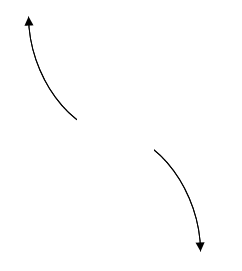
\includegraphics[width = 0.3\textwidth]{../Figures/polyEndBehaviorCopyAA.png}\item 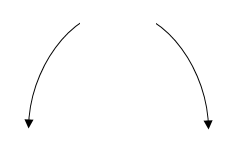
\includegraphics[width = 0.3\textwidth]{../Figures/polyEndBehaviorCopyBA.png}\item 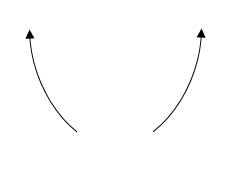
\includegraphics[width = 0.3\textwidth]{../Figures/polyEndBehaviorCopyCA.png}\item 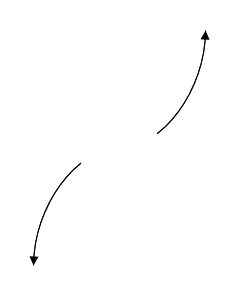
\includegraphics[width = 0.3\textwidth]{../Figures/polyEndBehaviorCopyDA.png}\end{multicols}\item None of the above.
\end{enumerate} }
\litem{
Construct the lowest-degree polynomial given the zeros below. Then, choose the intervals that contain the coefficients of the polynomial in the form $ax^3+bx^2+cx+d$.\[ \frac{-1}{4}, \frac{-1}{5}, \text{ and } 5 \]\begin{enumerate}[label=\Alph*.]
\item \( a \in [15, 26], b \in [-94, -89], c \in [-48, -42], \text{ and } d \in [0, 6] \)
\item \( a \in [15, 26], b \in [-101, -98], c \in [3, 5], \text{ and } d \in [0, 6] \)
\item \( a \in [15, 26], b \in [-94, -89], c \in [-48, -42], \text{ and } d \in [-6, 2] \)
\item \( a \in [15, 26], b \in [90, 92], c \in [-48, -42], \text{ and } d \in [0, 6] \)
\item \( a \in [15, 26], b \in [-109, -104], c \in [45, 48], \text{ and } d \in [-6, 2] \)

\end{enumerate} }
\litem{
Which of the following equations \textit{could} be of the graph presented below?
\begin{center}
    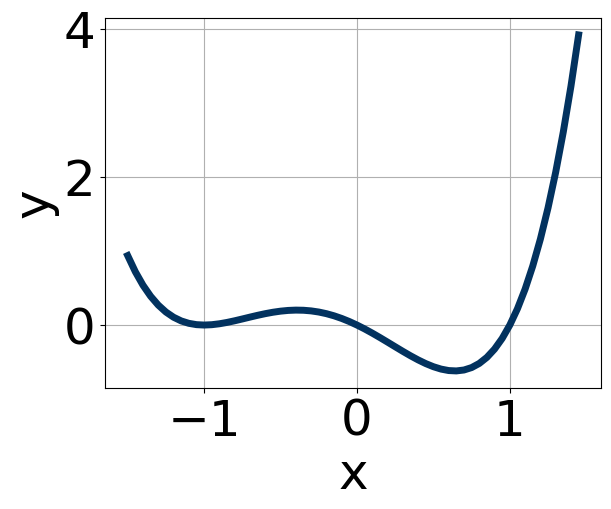
\includegraphics[width=0.5\textwidth]{../Figures/polyGraphToFunctionA.png}
\end{center}
\begin{enumerate}[label=\Alph*.]
\item \( -5x^{10} (x - 1)^{8} (x + 2)^{7} \)
\item \( -9x^{5} (x - 1)^{4} (x + 2)^{4} \)
\item \( -8x^{7} (x - 1)^{10} (x + 2)^{11} \)
\item \( 17x^{10} (x - 1)^{6} (x + 2)^{6} \)
\item \( 4x^{4} (x - 1)^{10} (x + 2)^{9} \)

\end{enumerate} }
\end{enumerate}

\end{document}